\question{Электронный прожектор. Формирование тонкого электронного пучка в
  прожекторе}

Для формирования аксиально-симметричных электронных потоков используются
триодные системы~-- т.~н. электронные прожекторы. Они состоят из катода,
эмитирующего электроны, модулятора, играющего роль сетки, и системы электродов с
потенциалами, отличными от потенциалов катода, необходимых для фокусировки
электронного потока (рис.~\pic{23scheme}). В качестве модулятора обычно
используется линза-диафрагма с круглым отверстием.
\begin{figure}[h!]
  \center
  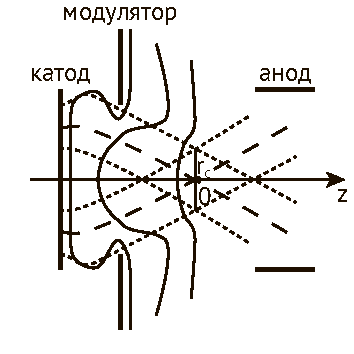
\includegraphics[width=.3\textwidth]{23_scheme} \hspace{1em}
  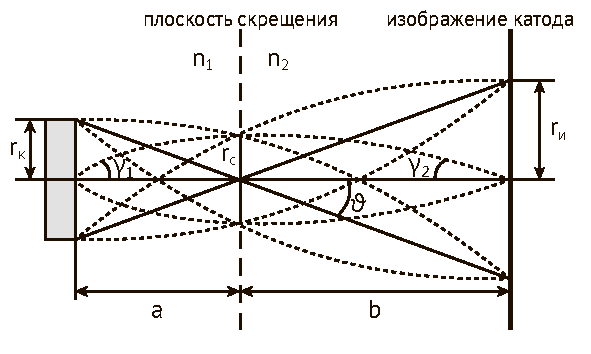
\includegraphics[width=.5\textwidth]{23_paths} \\
  \parbox{.3\textwidth}{\caption{Схема прожектора и картина поля в прикатодной
    области} \label{pic23scheme}} \hspace{1em}
  \parbox{.5\textwidth}{\caption{Формирование скрещенных траекторий в
    электронном прожекторе} \label{pic23paths}}
\end{figure}

Пусть электроны покидают катод с начальной скоростью, определяемой температурой
катода: \( v_0 = 2\sqrt{kT / m} \). Этой скорости можно сопоставить некоторый
эквивалентный потенциал: \( U_\text{э} = mv_0^2 / (2 \cdot e) \).

Будем считать, что все электроды являются телами вращения и обладают осевой
симметрией, следовательно, картина поля на рисунке~\pic{23scheme} является
сечением в одной из плоскостей, и движение электронов будет происходить только
в этой плоскости.

При отсутствии начальных скоростей электроны имели бы траектории, близкие к
силовым линиям электростатического поля и пересекали бы ось \( z \) в одной
точке (рис.~\pic{23scheme}, штриховые линии). При наличии же начальных скоростей
электроны пересекают ось в некотором интервале \( \D z \). В этом случае в
плоскости \( z = 0 \) траектории лежат внутри круга радиуса \( r_c \),
называемого радиусом скрещения.

Определим его величину и распределение плотности тока внутри него.

\subquestion{Определения радиуса скрещения}
Для определения радиуса скрещения воспользуемся теоремой Лагранжа-Гельмгольца,
которая для световых лучей имеет следующий вид:
\begin{equation}
  R_1 n_1 \gamma_1 = R_2 n_2 \gamma_2,
  \label{eq23optic}
\end{equation}
где \( R_1 \), \( R_2 \)~-- удаление точек объекта и изображения от оси;
\( n_1 \), \( n_2 \)~-- показатели преломления сред; \( \gamma_1 \),
\( \gamma_2 \)~-- апертурные углы (рис.~\pic{23theorem}).
\begin{figure}[hb!]
  \center
  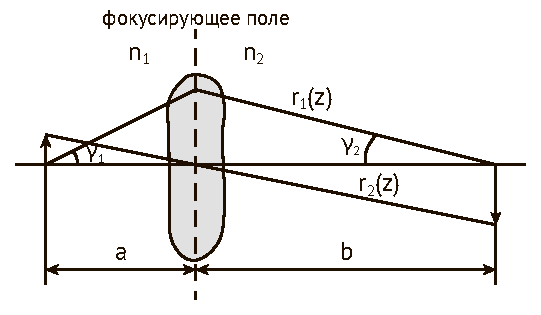
\includegraphics[width=.4\textwidth]{23_theorem}
  \caption{К выводу теоремы Лагранжа-Гельмгольца}
  \label{pic23theorem}
\end{figure}

Допустим, что существует два независимых решения \( r_1(z) \) и \( r_2(z) \)
основного уравнения параксиальной электроники \eqref{eq09paraxial}. Подставим
их в \eqref{eq09equation}:
\[
  \sqrt{U_0} \der{}{z} \left( \sqrt{U_0}\ \der{r_1}{z} \right) =
    -\frac{U_0'' r_1}{4}, \qquad
  \sqrt{U_0} \der{}{z} \left( \sqrt{U_0}\ \der{r_2}{z} \right) =
    -\frac{U_0'' r_2}{4}.
\]

Домножим первое соотношение на \( r_2 \), второе~-- на \( r_1 \) и вычтем второе
из первого. Получим
\[
  0 = \sqrt{U_0} \left[ r_2 \der{}{z} \left( \sqrt{U_0}\ \der{r_1}{z} \right) -
    r_1 \der{}{z} \left( \sqrt{U_0}\ \der{r_2}{z} \right) \right] =
    \der{}{z} \left[ \sqrt{U_0} \left( r_2 \der{r_1}{z} - r_1 \der{r_2}{z}
    \right) \right].
\]

Интегрирование последнего дает
\begin{gather*}
  \sqrt{U_0} \left( r_2 \der{r_1}{z} - r_1 \der{r_2}{z} \right) = \const,
    \text{ или } \\
  \sqrt{U_a} \Big[ r_2(z_a) r_1'(z_a) - r_1(z_a) r_2'(z_a) \Big] =
    \sqrt{U_b} \Big[ r_2(z_b) r_1'(z_b) - r_1(z_b) r_2'(z_b) \Big],
\end{gather*}
где штрихи означают производные по \( z \), индексы \( a \) и \( b \) означают
пространство до и после линзы соответственно.

Если выбрать решение таким, чтобы \( r_1(z_a) = r_2(z_b) = 0 \) (случай, когда в
области линзы вторая производная положительная), получим
\begin{equation}
  \sqrt{U_a} r_2(z_a) r_1'(z_a) = \sqrt{U_b} r_2(z_b) r_1'(z_b).
  \label{eq23electronic}
\end{equation}

Тогда \( r_1'(z_{a,\,b}) \approx \gamma_{1,\,2} \) для малых апертурных углов в
параксиальной области, \( r_2(z_{a,\,b}) = R_{1,\,2} \),
\( \sqrt{U_{a,\,b}} = n_{1,\,2} \) и \eqref{eq23electronic} приобретает вид
\eqref{eq23optic}.

При больших апертурных углах , когда нарушается параксиальность траекторий
электронов, пользуются условием синусов Аббе:
\begin{equation}
  R_1 n_1 \sin\gamma_1 = R_2 n_2 \sin\gamma_2,
  \label{eq23Abbe}
\end{equation}
получаемое из \eqref{eq23electronic} представлением производных в виде синусов:
\( r_1'(z_{a,\,b}) \approx \sin\gamma_{1,\,2} \). В соответствии с
рисунком~\pic{23paths} \( r_1 \) и \( r_2 \)~-- радиусы катода \( r_\text{к} \)
и изображения \( r_\text{и} \) соответственно. Радиус скрещения равен
\( r_c = b \cdot \tg\gamma_2 \), а радиус изображения~--
\( r_\text{и} = b \cdot \tg\theta \) (рис.~\pic{23paths}).

Ограничимся малыми углами (\( \sin\gamma_2 \approx \tg\gamma_2 \)), тогда из
\eqref{eq23Abbe} следует
\[
  r_\text{и} = \frac{r_\text{к} n_1 \sin\gamma_1}{n_2 \tg\theta}.
\]

Учитывая, что показатель преломления в плоскости катода
\( n_1 \approx \sqrt{U_\text{э}} \), а в плоскости скрещения
\( n_2 \approx \sqrt{U_0} \) (\( U_0 \)~-- потенциал в плоскости изображения),
получим
\begin{equation}
  r_c = \frac{r_\text{к}}{\tg\theta} \sqrt{\frac{U_\text{э}}{U_0}} \sin\gamma_1
    = a\sqrt{\frac{U_\text{э}}{U_0}} \sin\gamma_1.
  \label{eq23rc}
\end{equation}
Здесь \( a \)~-- расстояние от поверхности катода до плоскости скрещения. Как
видно, в первом приближении радиус скрещения не зависит от площади катода
\( S_\text{к} \).

\subquestion{Определение плотности тока в плоскости z = 0}

Электроны, испускаемые катодом, имеют распределение по скоростям; при этом
минимальная величина их энергии при вылете должна превышать работу выхода из
катода.

Применим распределение Максвелла, которое для количества электронов, вылетающих
в единицу времени с единицы площади поверхности катода нормально к ней,
приходящихся на единицу телесного угла и имеющих энергию от \( eU \) до
\( e(U + dU) \), задается соотношением
\begin{equation}
  N(U) dU = N_0 \frac{eU}{kT} \exp\left( -\frac{eU}{kT} \right)\,d\frac{eU}{kT},
  \label{eq23Maxw}
\end{equation}
где \( N_0 \)~-- величина, характеризующая количество электронов всех возможных
энергий, испускаемых катодом в единицу времени с единицы площади поверхности
нормально к ней в единице телесного угла. Ее можно определить из плотности тока
эмиссии с катода:
\begin{equation}
  j_\text{к} = e\pi N_0.
  \label{eq23jk}
\end{equation}

Испускание электронов с катода подчиняется закону Ламберта:
\begin{quote}
  \emph{ток электронов в любом направлении пропорционален косинусу угла между
  нормалью к поверхности катода и данным направлением.}
\end{quote}

Тогда ток в пределах телесного угла от \( \gamma \) до
\( \gamma + d\gamma \) будет равен
\[
  dI_\gamma = 2\pi S_\text{к}eN \sin\gamma \cos\gamma \,d\gamma.
\]

В плоскости скрещения через кольцо, заключенное между окружностями с радиусами
\( r_c \) и \( r_c + dr_c \), чему соответствует интервал углов от
\( \gamma_1 \) до \( \gamma_1 + d\gamma_1 \), будет проходить ток
\[
  dI_{\gamma_1} = 2\pi S_\text{к}eN_1 \sin\gamma_1 \cos\gamma_1 \,d\gamma_1.
\]
Здесь \( N_1 \)~-- количество электронов, эмитируемых катодом с энергиями в
интервале \( \big[ eU_\text{э},\ e(U_\text{э} + dU_\text{э}) \big] \).

Тогда плотность тока в кольцевой зоне равна
\[
  j_r = \der{I_{\gamma_1}}{(\pi r_c^2)} = \frac{S_\text{к} e N_1 \sin\gamma_1
    \cos\gamma_1 \,d\gamma_1}{r_c\,dr_c},
\]
или, с учетом \eqref{eq23rc},
\[
  j_r = \frac{S_\text{к} N_1 eU_0}{a^2 U_\text{э}}.
\]

Суммируем все плотности токов, протекающих через кольцевые участки плоскости,
образуемых электронами с энергиями, большими \( eU_\text{э} \):
\[
  j = \frac{S_\text{к} e}{a^2} \int\limits_{U_\text{э}}^\infty
    \frac{U_0}{U_\text{э}} N(U_\text{э})\,dU_\text{э}.
\]

Заменяя \( U_\text{э} \) из \eqref{eq23rc} при условии \( \sin\gamma_1 = 1 \),
используя \eqref{eq23Maxw} и интегрируя, получаем выражение для плотности тока
в плоскости скрещения:
\[
  j = \frac{eS_\text{к} N_0}{a^2} \left( 1 + \frac{eU_0}{kT} \right)
    \exp{-\frac{eU_0}{kT}\frac{r^2}{a^2}}.
\]

Заменяя \( a \) на \( r_\text{к}\sin\theta \), считая для малых углов синус и
тангенс равными и подставляя \( N_0 \) из \eqref{eq23jk}, получаем формулу
Ленгмюра для плотности тока в центре скрещения (\( r = 0 \)):
\[
  j_0 = j_\text{к} \left( \frac{eU_0}{kT} + 1 \right) \sin^{-2}\theta.
\]
